\section{Appendix}

\subsection{URLs}
Project Links: 

\href{https://bitbucket.org/comp90024team39/comp90024-a2/src/master/}{Bitbucket Repository}

(https://bitbucket.org/comp90024team39/comp90024-a2/src/master/)

\href{https://youtu.be/574I-g7GSGI }{Production Deployment Video} 

(https://youtu.be/574I-g7GSGI )

\href{https://youtu.be/cqmxZdLdOyk}{Product Demo Video} 

(https://youtu.be/cqmxZdLdOyk) \\

This application supports following URLs:
\begin{itemize}
    \item Page navigation: \url{http://172.26.129.79/analyser/}
    \item Tweets related: \url{http://172.26.129.79/analyser/tweets/}
    \begin{itemize}
        % \item Get single tweet:\\ \url{http://172.26.129.79/analyser/tweets/:id}
        \item Get the stats of tweets\\
        \url{http://172.26.129.79/analyser/tweets/stats/}
        \item Get the stats of sport related tweets\\
        \url{http://172.26.129.79/analyser/tweets/sports}
    \end{itemize}
    \item User related: \url{http://172.26.129.79/analyser/users/}
    \begin{itemize}
        \item Get stats of users\\
        \url{http://172.26.129.79/analyser/users/stats}
        \item Get the sport enthusiasts rank\\
        \url{http://172.26.129.79/analyser/users/rank/}
    \end{itemize}
    \item Sport related: \url{http://172.26.129.79/analyser/sports/}
    \begin{itemize}
        \item Get the stats of sports\\
        \url{http://172.26.129.79/analyser/sports/stats_all}
        \item Get the stats of sports in specific yearly time interval (from 2019 to 2021)\\
        \url{http://172.26.129.79/analyser/sports/<year>-<year>}
        For example: \url{http://172.26.129.79/analyser/sports/2019-2020/}
        \item Get the top 3 sports\\
        \url{http://172.26.129.79/analyser/sports/rank_top3}
    \end{itemize}
    \item Job control: \url{http://172.26.129.79/analyser/jobs/}
    \begin{itemize}
        \item Get all jobs status\\
        \url{http://172.26.129.79/analyser/jobs/all/}
        \item Start twitter harvester\\
        \url{http://172.26.129.79/analyser/jobs/search}
        \item Start updating users timeline\\
        \url{http://172.26.129.79/analyser/jobs/update}
        \item Start streaming tweets\\
        \url{http://172.26.129.79/analyser/jobs/stream}
        \item Get the sport enthusiasts rank\\
        \url{http://172.26.129.79/analyser/jobs/user_rank}
    \end{itemize}
    \item Initialise couchdb
    \url{http://172.26.129.79/analyser/initialiser}
\end{itemize}

\subsection{User Guide}

This section describes the testing steps. 

\subsubsection{Logins}

CouchDB: user:pass

Portainer: admin:password

HAProxy: admin:password

\subsubsection{Installation}

\textbf{To install the system: }

\begin{itemize}
    \item Clone the repository and change directory to $./deployment$.
    \item Prepare a clean project unimelb-comp90024-2021-grp-39 on MRC. if you want to use other projects, update unimelb-comp90024-2021-grp-39-openrc.sh content with your openrc.sh code. 
    \item Run \href{https://bitbucket.org/comp90024team39/comp90024-a2/src/master/deployment/init.sh}{./init.sh}
    \item enter the password from MRCpassword.txt or your own. 
    \item Go to the home page (any instance IP)
    \item Go to Manage
    \item Set up as local swarm
\end{itemize}

\\

\textbf{To scale up instances,}

\begin{itemize}
    \item Inspect \href{https://bitbucket.org/comp90024team39/comp90024-a2/src/master/deployment/host_vars_scale.yaml}{./host\_vars\_scale.yaml} and update the details of the new resources
    \item Run \href{https://bitbucket.org/comp90024team39/comp90024-a2/src/master/deployment/init.sh}{./scale.sh}
    \item Enter the master password from MRCpassword.txt or your own
    \item Go to the home page (any instance IP) 
    \item Go to ``Manage" from the bottom left of home.
    \item Portainer login is admin:password. 
    \item Go to Services 
    \item Scale up services by an appropriate level.  
\end{itemize}

\\

\textbf{To scale up services,} 
\begin{itemize}
    \item Go to Manage page (Portainer) from home
    \item Go to Services 
    \item Click Scale
    \item Enter the number of nodes
    \item click tick
\end{itemize}

An important note is that CouchDB ideally needs at least 2 cores to run properly, as mentioned by its developer. \\

\textbf{To check where the containers are distributed: }

\begin{itemize}
    \item Go to Manage page (Portainer)
    \item Go to Dashboard 
    \item Click ``Go to the visualizer"
\end{itemize}

\subsubsection{Testing}

If charts are missing on the Statistics page, please refresh the page and the charts will load. 

\textbf{To test the harvesters,}

\begin{itemize}
    \item Enter the number of users per city on the home page bottom panel
    \item Click Add New Users
\end{itemize}

The more users exist in the database, the harder it is to get new users. Typically a batch job of 1 new user per city consumes 15-30 minutes to finish.\\

\textbf{To add more tweets,}

\begin{itemize}
    \item Click Search User Tweets
\end{itemize}

Normally this will search for the user timeline for all the users who have not been harvested for over 7 days. Since a lot of user data were collected early, this job will run for a long time. The tester may need to wait 10-20 minutes to see the first update. 

Moreover, the tokens being used might be limited at this stage since the beginning, so the wait time on new data collection is not guaranteed. 

When stopping the jobs, it may take a few minutes to completely stop. 

We had planned to partition the database by cities, but only realised the 10G partition size limitation when most data is in place. It is estimated to take 2 days to migrate the partition method and the relevant code. It is not a difficult job but CouchDB will consume 10-15 hours to rebuild the views. Due to the limited time-frame, we have left it as is. If the user continues to harvest a large amount of data, it may potentially hit the size limit. 


\subsubsection{Troubleshooting}

If CouchDB services are restarted or you see ``Failed to load database" error run \href{https://bitbucket.org/comp90024team39/comp90024-a2/src/master/deployment/recluster-couchdb.sh}{recluster-couchdb.sh} 

\subsubsection{UI}
Home page (Fig.\ref{UserGuid1}, \ref{UserGuid2} link: \url{http://172.26.129.79/home/}): On the left side is the navigator. It is composed by two parts, \textcircled{1} Page Navigator and \textcircled{2} Management Menu. Users can switch to other pages through \textcircled{1}Page navigator for more information extracted from harvest data, admin can manage the instances (\url{http://172.26.129.79:9000}), HAProxy (\url{http://172.26.129.79/haproxy-admin/}), Spark (\url{http://172.26.129.79:8080}) and CouchDB (\url{http://172.26.129.79:5984}) with the \textcircled{2}Management menu. \textcircled{3} Twitter Harvest Status shows the Twitter harvester status in instances. There are two statuses. When the job is running, the status will be displayed as running, and idle means the job is ready to start. Users can start the job with the \textcircled{4} Twitter Harvest Job Control Module. The control buttons will be enabled if the corresponding Twitter harvest status is idle. The search button means searching for new tweets. Before clicking the search button, users need to input the number of users they want to search in the input box. Click the stream button will start harvesting the most recent tweets, and the update button is to update users’ timelines.
\begin{figure*}
\centerline{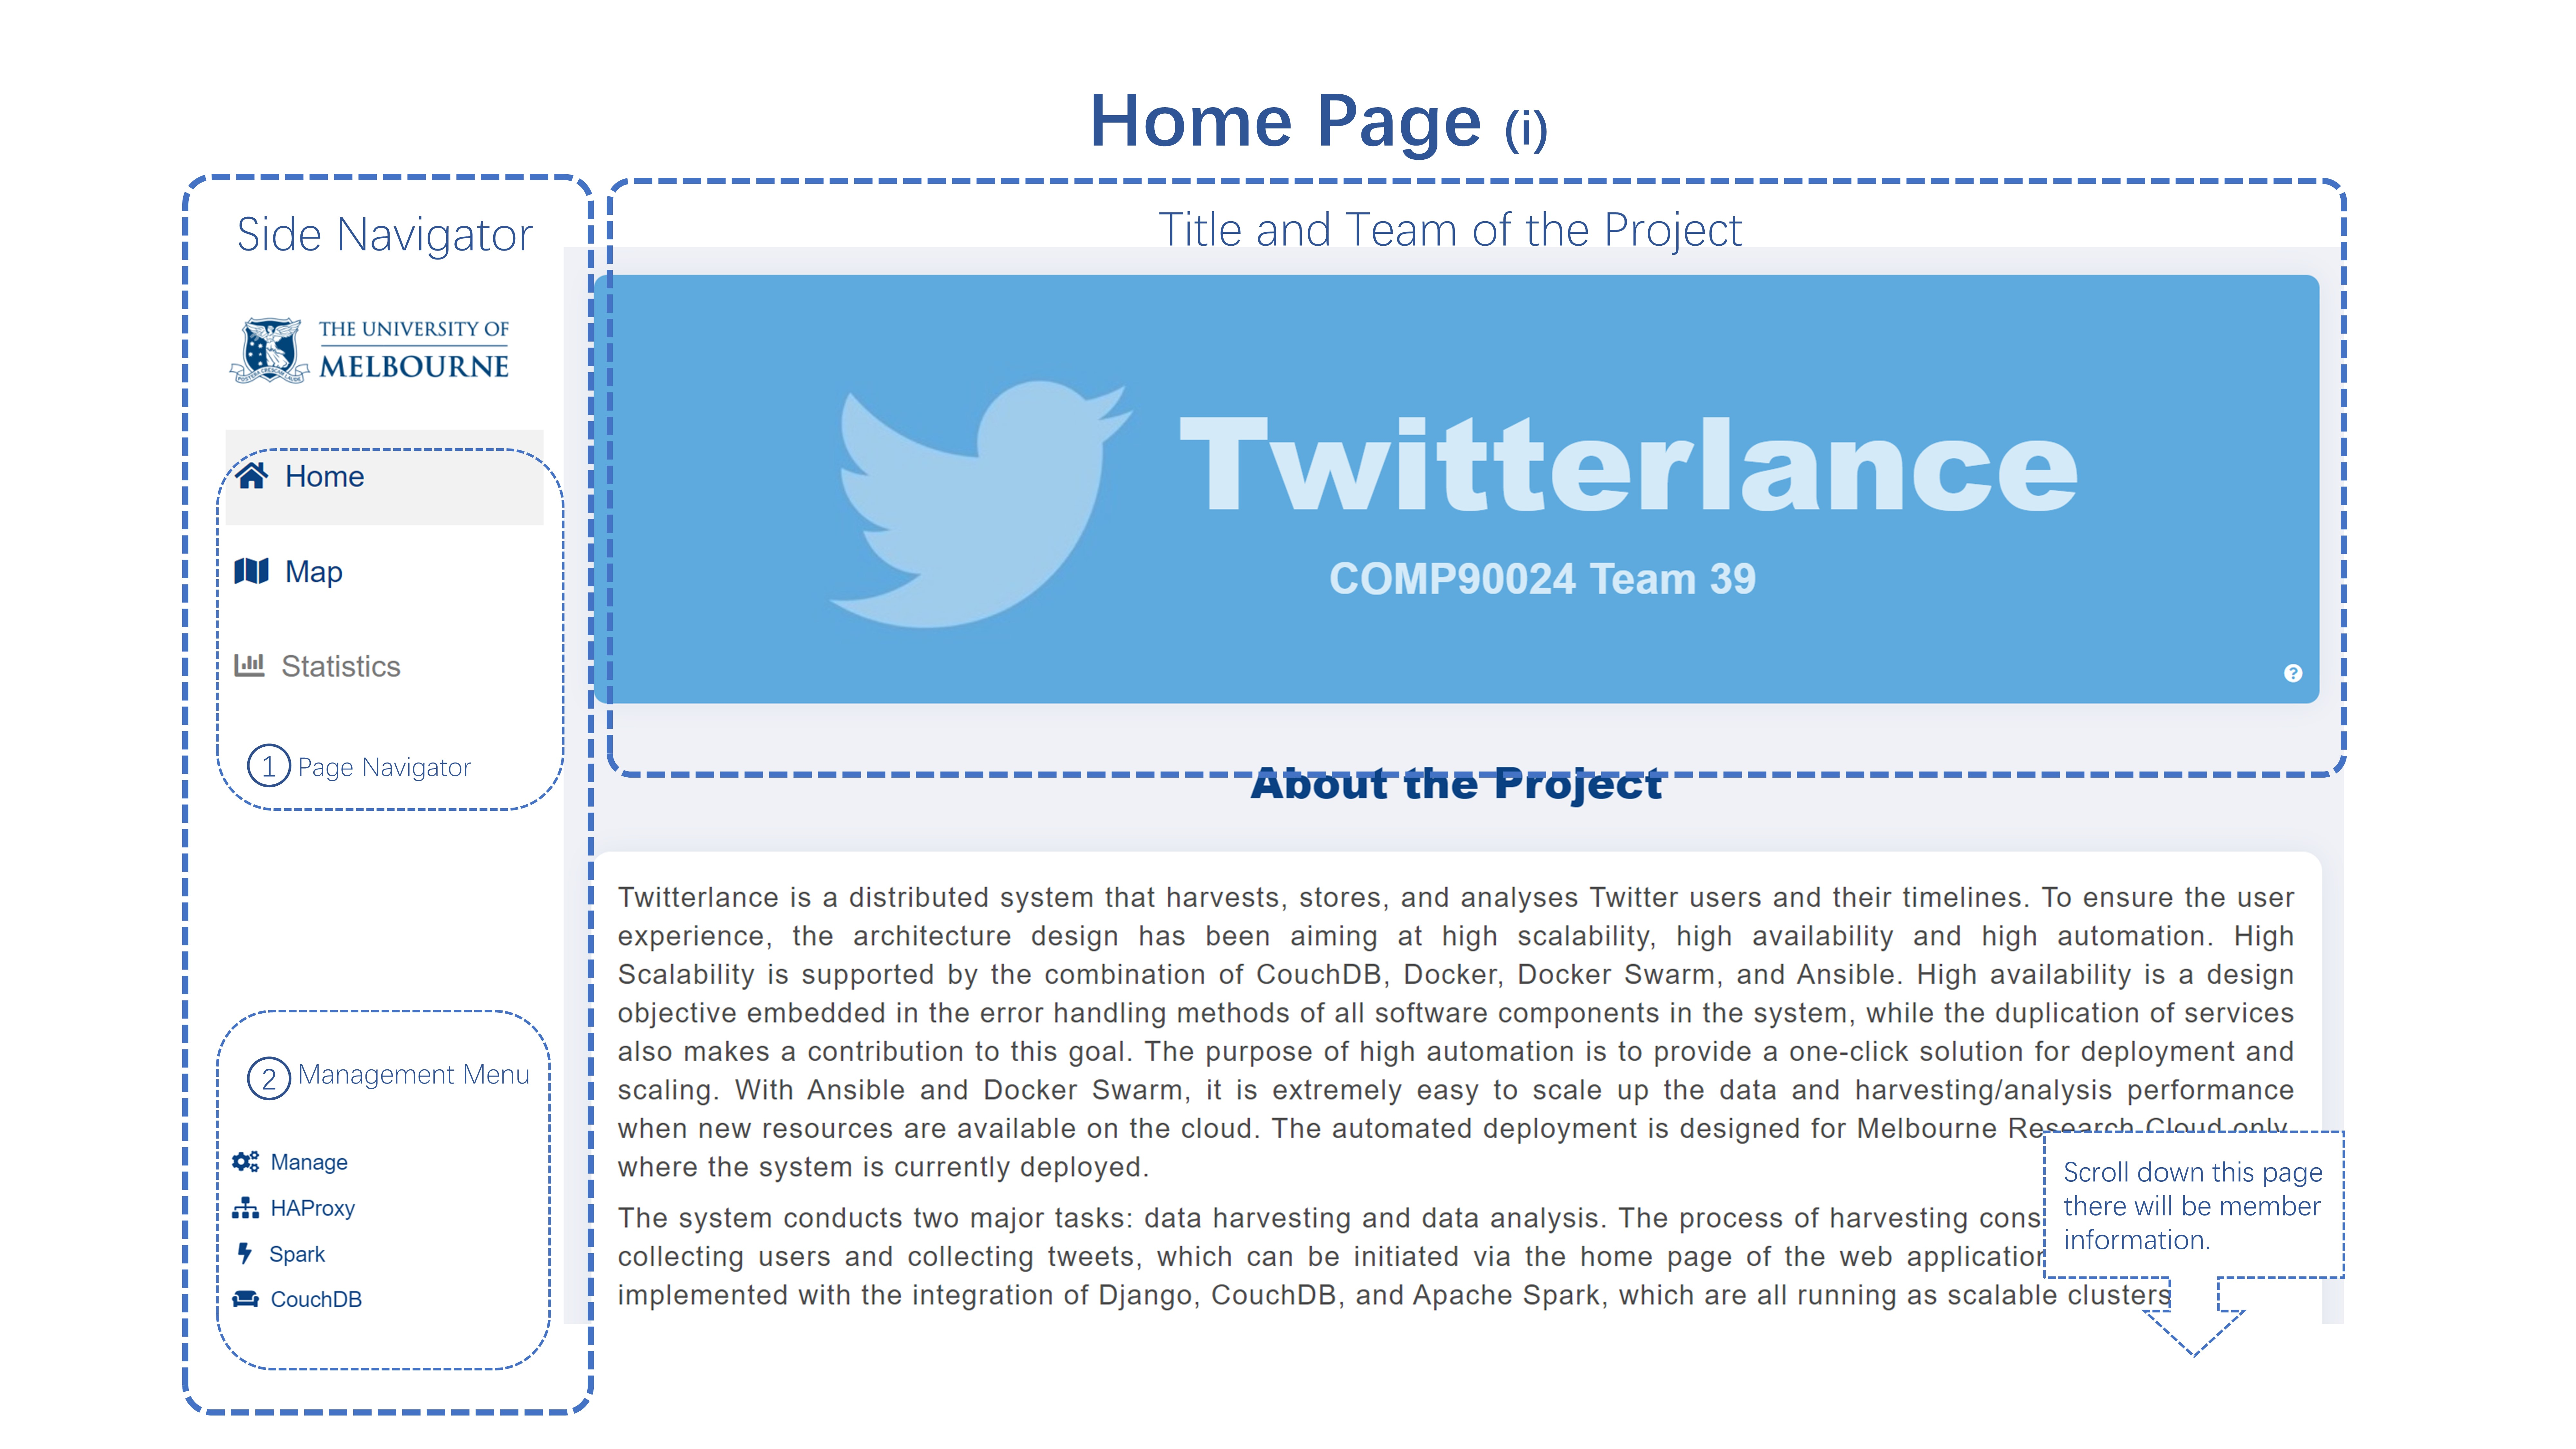
\includegraphics[width=7in]{Figures/UserGuid1.JPG}}
\caption{Home Page (i)}
\label{UserGuid1}
\end{figure*}

\begin{figure*}
\centerline{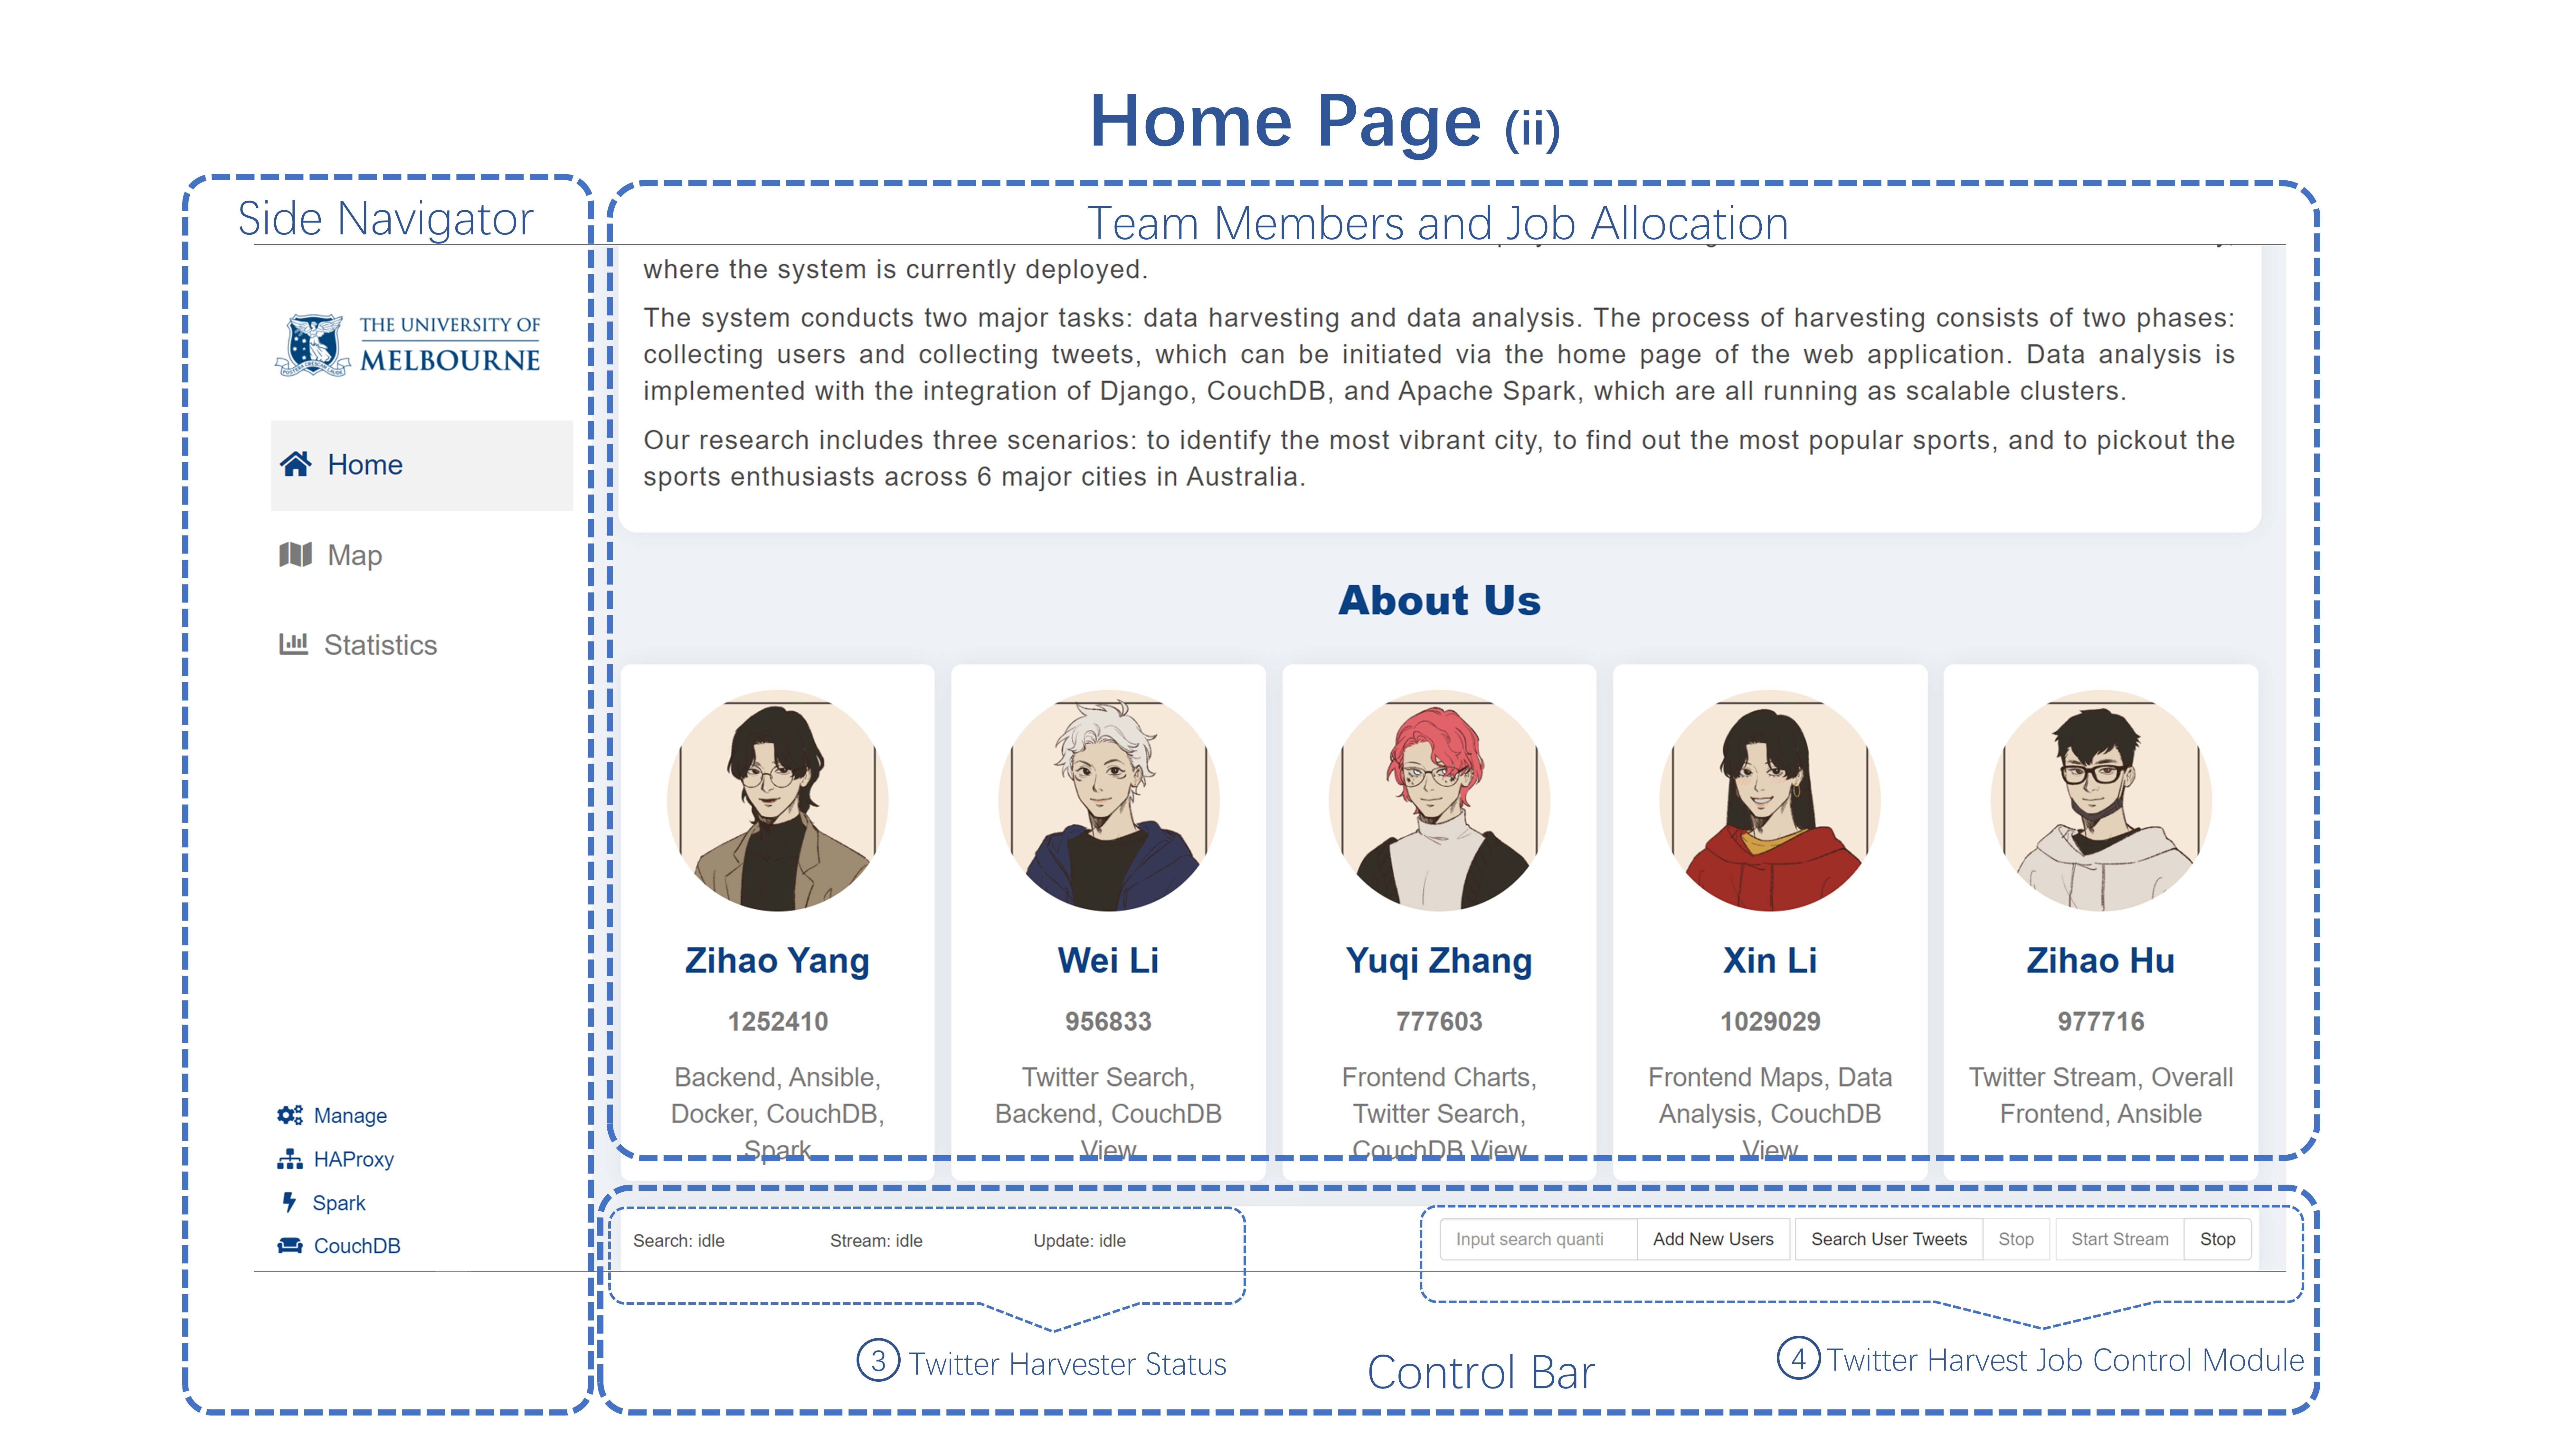
\includegraphics[width=7in]{Figures/UserGuide2.JPG}}
\caption{Home Page (ii)}
\label{UserGuid2}
\end{figure*}

Map page (Fig.\ref{UserGuid3} link: \url{http://172.26.129.79/map/}): Users can quickly locate their interested city with the \textcircled{7} Search Bar on the top right of the page. (For the limit of time and resources we only display data of six cities.) \textcircled{6}Interested Cities will be displayed on the map with blue circles. The radius of circles is decided by the quantities of tweets harvested in corresponding cities. When the mouse hovers on one of the interested cities, \textcircled{5}Statistics of the city will be displayed on the left side of the map page.

\begin{figure*}
\centerline{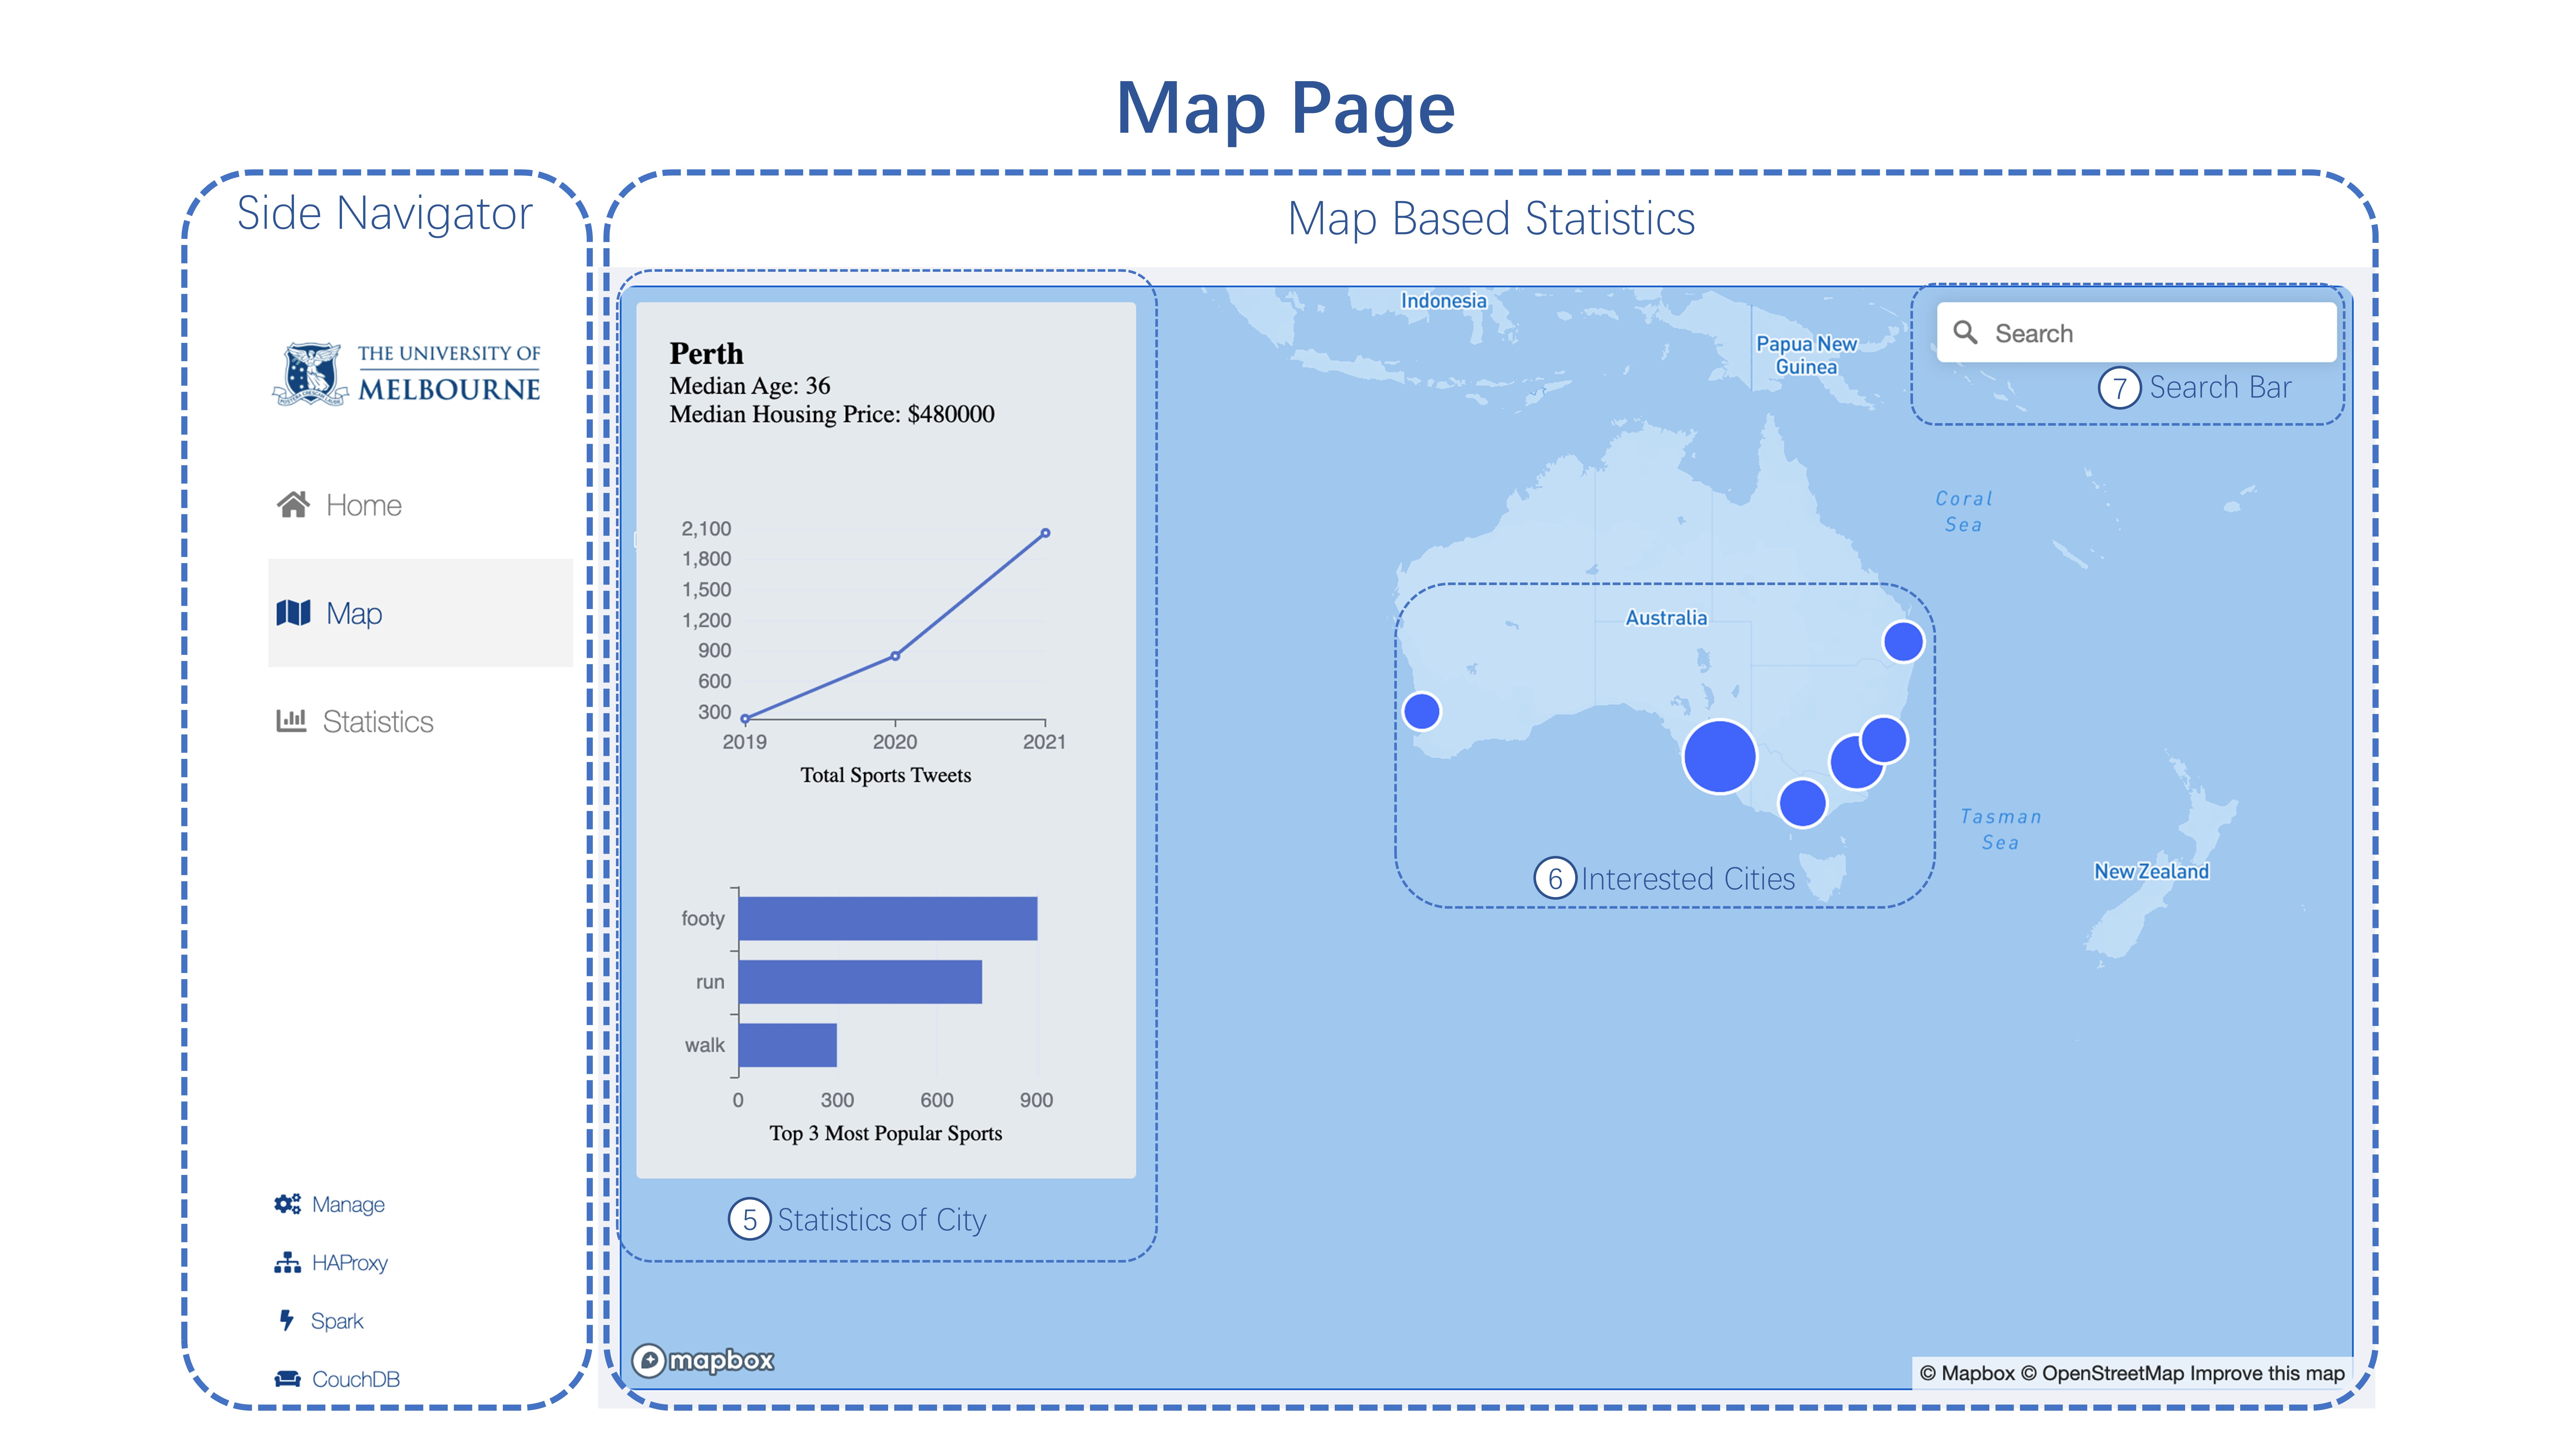
\includegraphics[width=7in]{Figures/UserGuide3.JPG}}
\caption{Map Page}
\label{UserGuid3}
\end{figure*}

Statistics page (Fig.\ref{UserGuid4} link: \url{http://172.26.129.79/statistics/}): \textcircled{8}Overall statistics shows: a) the total number of users we searched and stored in the database, b) the total number of tweets we harvested from users, c) the total number of sport-related tweets. Users can switch to different charts through the \textcircled{9} Chart Tab. When the chart tab is activated, the color will be changed from blue to white. Sex $\&$ Age tab is linked to bar-charts of the gender ratio and median age across six cities. Work $\&$ Study tab is linked to the bar charts of the unemployment rate and Education level across six cities. Income $\&$ Freq tab is linked to the bar-charts of median-income and tweets frequencies across six cities. More scenarios will be displayed if Users scroll down this page.

\begin{figure*}
\centerline{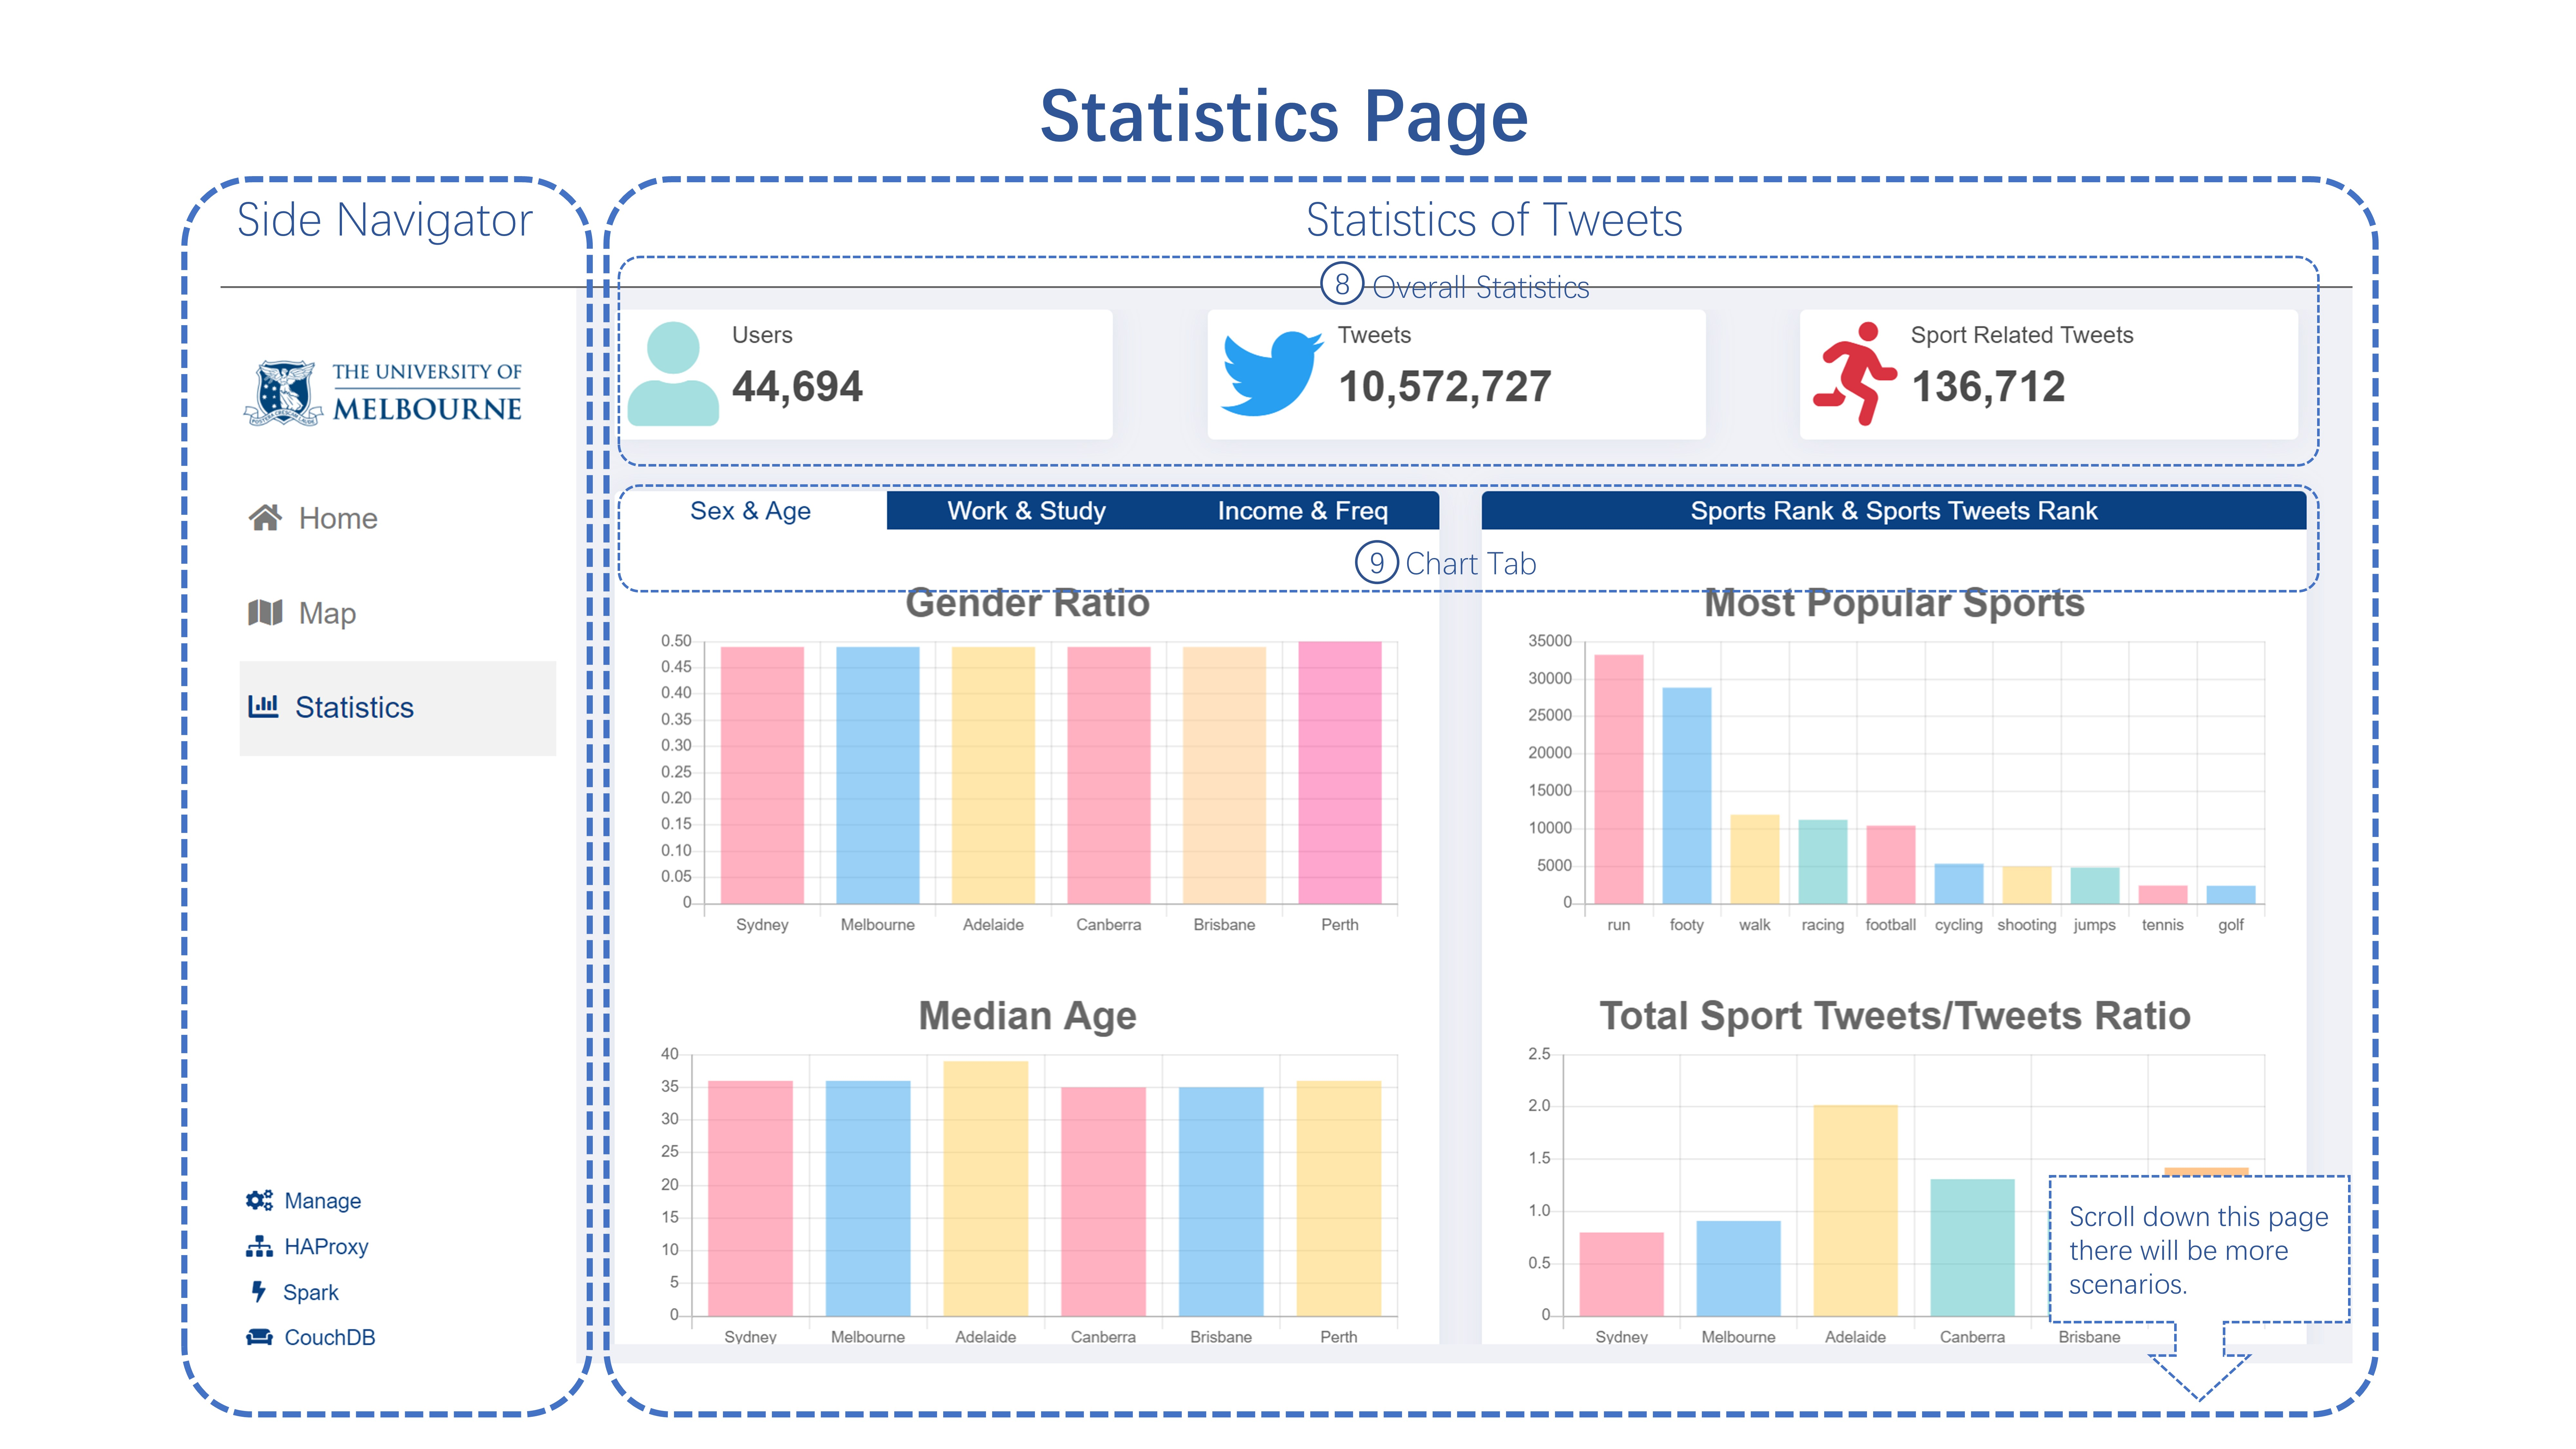
\includegraphics[width=7in]{Figures/UserGuide4.JPG}}
\caption{Statistics Page}
\label{UserGuid4}
\end{figure*}
\newpage

\subsection{Pseudo code}
\begin{algorithm}[h!]
\caption{Search User Algorithm}
\SetAlgoLined
\SetKwProg{Fn}{Function}{}{end}
\SetKwProg{try}{try}{:}{}
\SetKwProg{except}{except}{:}{}
\Fn{search\_user(query: str, city: str, api, rate\_limit = 10, latest\_id = None, count = 0)}{
\tcc{query = whitespace, used in Twitter API}
\tcc{city = the full name of city, used in structure user profile}
\tcc{api = Twitter API token, user in Twitter API}
\tcc{rate\_limit = how many users the system want to add in this city}
\tcc{latest\_id = the oldest tweet index in a batch tweets, used in breakpoint retransmission}
\tcc{count = how many users have been added, used in breakpoint retransmission}
Initiation;\\
get user list from users database in CouchDB;\\
get geocode of the city from cities database in CouchDB;\\
\eIf{Twitter API works}{
pass\;
}{
\KwRet \tcc{move to next token}
}
\While{count does not meet the rate\_limit}{
\try{}{
yield a batch of tweets from search API;\\
}
\except{}{
\KwRet False, maxid, count \tcc{move to next token}
}
\For{tweet in tweets}{
\eIf{the user not in the user list}{
append the user to save list\;
}{
pass
}
}
\try{}{
feed the save list to CouchDB;\\
}
\except{}{
retry for 5 times maximally;
}
\eIf{success to save users}{
get the maxid of that batch;\\
count += the length of the save list;\\
}{
continue in this batch
}
}
\KwRet True, None, count
}
\label{algorithm: searchuser}
\end{algorithm}

\begin{algorithm}[h!]
\caption{Run Search User Algorithm}
\SetAlgoLined
\SetKwProg{Fn}{Function}{}{end}
\Fn{run\_search(i: int)}{
\tcc{i = the rate\_limit fed from the frontend}
get cities from cities database in CouchDB;\\
get tokens from tokens database in CouchDB;\\
scale up and shuffle token list;\\

\For{city in cities}{
\For{token in tokens}{
get api from token list;\\
\eIf{search\_user returns True}{
break}{
continue to search from the returned maxid and count} 
}
}
}
\label{algorithm: runsearch}
\end{algorithm}

\begin{algorithm}[h!]
\caption{Run Update Timeline Algorithm}
\SetAlgoLined
\SetKwProg{Fn}{Function}{}{end}
\SetKwProg{try}{try}{:}{}
\SetKwProg{except}{except}{:}{}
\Fn{assign\_task()}{
\try{}{get user list from users database in CouchDB;\\}
\except{}{try again 10 mins latter} \tcc{wait for database compaction or view regenerating}
get the node list from nodes database in CouchDB;\\
find the index of current node;\\
evenly split the user list by the node number;\\
assign the node with sub\_user\_list corresponding to its index;\\
\KwRet sub\_user\_list
}
\Fn{run\_update()}{
get tokens from tokens database in CouchDB;\\
scale up and shuffle the token list; \tcc{expand the token pool}\\
assign\_task(); \tcc{assign task for one node}\\
\For{user in sub\_user\_list}{
\For{token in tokens}{
get api from token list;\\
\eIf{search\_tweets returns True}{
break}{
continue} 
}
}
}
\end{algorithm}

\begin{algorithm}[H]
\caption{Update Timeline Algorithm}
\SetAlgoLined
\SetKwProg{Fn}{Function}{}{end}
\SetKwProg{try}{try}{:}{}
\SetKwProg{except}{except}{:}{}
\Fn{search\_tweets(user: dict, api, timeline\_limit= 400)}{
\tcc{user = a dictionary, used in Twitter API}
\tcc{api = Twitter API token, user in Twitter API}
\tcc{timeline\_limit = how many new tweets the system want to add}
Initiation;\\
get user list from users database in CouchDB;\\
get geocode of the city from cities database in CouchDB;\\
\try{}{
yield a batch of tweets from search timeline API;\\
}
\except{}{
\KwRet False \tcc{move to next token}
}

\While{the length of save list of does not meet the timeline\_limit}{
\uIf{the length of the latest batch tweets = 0}{
break
}{
}
\uElseIf{the length of the latest batch tweets = 200}{
save the tweets into save list;\\
get the maxid of this batch;\\
\try{}{yield next batch of tweets from search timeline API;}
\except{}{\KwRet False}
}
\Else{
save the tweets into save list;\\
break;
}
}
\try{}{
feed the save list to CouchDB;\\
}
\except{}{
retry for 5 times maximally;
}
\eIf{success to save users}{
\KwRet True
}{
\KwRet False
}
}
\end{algorithm}


\begin{algorithm}[h!]
\caption{Stream tweets Algorithm}
\SetAlgoLined
\SetKwProg{Fn}{Function}{}{end}
\SetKwProg{try}{try}{:}{}
\SetKwProg{except}{except}{:}{}
\Fn{Stream\_tweets(cityBoundary: Json, api)}{
\tcc{user = a dictionary, used in Twitter API}
\tcc{cityBoundary = the boundaries of cities}
\tcc{api = Twitter API token, user in Twitter API}
Initiation;\\
get user list from users database in CouchDB;\\
get city boundaries Json file from Django;\\
\If{Twitter API works}{
pass\;
}
\While{True}{
\try{}{
yield a tweet from Stream API;\\
}
\except{}{
Stream harvester sleep for a while\;
}
\eIf{the tweet location in the target cities}{
\eIf{the user not in the user list}{
\tcc{stream harvester find a new user}
save the user to users database in CouchDB\;
append the user to user list\;
save the user timeline to tweets database in CouchDB\;
}{
\tcc{It is not a new user but stream API only get instant tweets}
save tweet to tweets database in CouchDB\;
}
}{
\KwRet False;
}
}
\KwRet True
}
\end{algorithm}


\begin{algorithm}[h!]
\caption{Run Stream tweets Algorithm}
\SetAlgoLined
\SetKwProg{Fn}{Function}{}{end}
\Fn{run\_stream()}{
get stream harvester job status from CouchDB\;
\eIf{status != `ready'}{
break
}{
set stream harvester job status to `running' in CouchDB\;
run Stream\_tweets\;
} 
}
\end{algorithm}